\subsection{UC4 - Apertura Cancello}
\begin{itemize}
    \item \textbf{Identificativo}: UC4
    \item \textbf{Nome}: apertura cancello
    \item \textbf{Descrizione grafica}:
\end{itemize}

\begin{figure}[h]
   \centering
   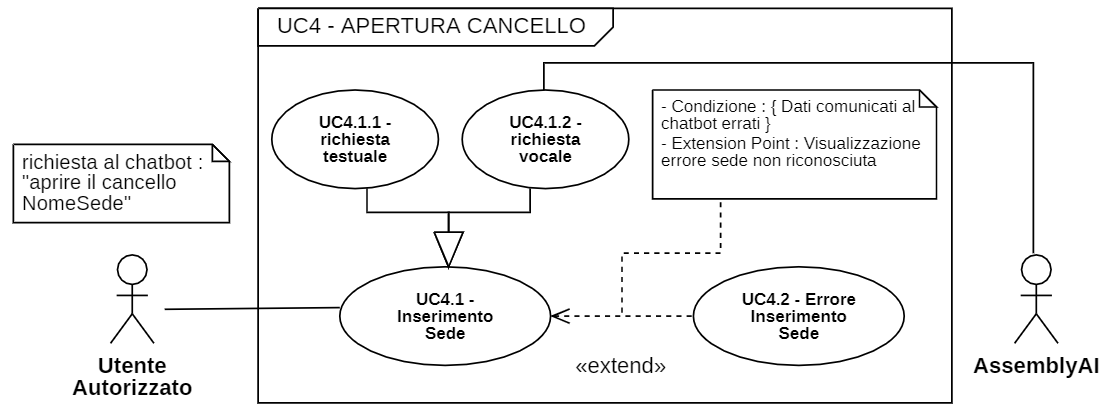
\includegraphics[scale=0.6]{images/UC4.png} 
   \caption{Descrizione grafica caso d'uso UC4}
\end{figure}


 \begin{itemize}
    \item \textbf{Attori}
 \begin{itemize} 
    \item \textit{Primari}: utente autorizzato
    \item \textit{Secondari}: non presenti
 \end{itemize}
 \item \textbf{Precondizione}: l'utente è autorizzato e si trova nell'interfaccia del chatbot.
 \item \textbf{Postcondizione}: il chatbot risponde alla richiesta dell'utente e invia la richiesta di apertura del cancello.
 \item \textbf{Scenario principale}: l'utente autorizzato richiede l'apertura del cancello, specificando la sede (UC4.1).
 \item \textbf{Estensioni}: 
 \begin{itemize} 
    \item il chatbot comunica all'utente che la sede specificata non è stata trovata (UC4.2).
 \end{itemize}
\end{itemize}
\newpage
\subsubsection{UC4.1 - Inserimento Sede}
\begin{itemize}
    \item \textbf{Identificativo}: UC4.1
    \item \textbf{Nome}: inserimento sede
    \item \textbf{Descrizione grafica}: (approfondita in UC4)
    \item \textbf{Attori}
 \begin{itemize} 
    \item \textit{Primari}: utente autorizzato 
    \item \textit{Secondari}: non presenti
 \end{itemize}
 \item \textbf{Precondizione}: l'utente ha comunicato al chatbot la richiesta di apertura del cancello di una sede.
 \item \textbf{Postcondizione}: il chatbot inoltra la richiesta per la sede specificata.
 \item \textbf{Scenario principale}: il chatbot chiede all'utente di specificare di quale sede vuole aprire il cancello. L'utente comunica al chatbot la sede tramite messaggio testuale (UC4.1.1) o vocale (UC4.1.2).
\item \textbf{Estensioni}: 
 \begin{itemize} 
    \item il chatbot comunica all'utente che la sede specificata non è stata trovata (UC4.2).
 \end{itemize}
\end{itemize}

\paragraph{UC4.1.1 - Richiesta Testuale}
\begin{itemize}
   \item \textbf{Identificativo}: UC4.1.1
   \item \textbf{Nome}: Richiesta testuale
   \item \textbf{Descrizione grafica}: (approfondita in UC4)
   \item \textbf{Attori}:
   \begin{itemize} 
       \item \textit{Primari}: utente autorizzato
       \item \textit{Secondari}: non presenti
   \end{itemize}
       \item \textbf{Precondizione}: l'utente si è autenticato al sistema e ha richiesto di voler aprire il cancello di una sede. 
       \item \textbf{Postcondizione}: l'utente fornisce il nome della sede della quale voler aprire il cancello.
    \item \textbf{Scenario principale}: 
       \begin{itemize}
           \item L'utente ha effettuato l'accesso al sistema 
           \item L'utente fornisce tramite input testuale il nome della sede, di cui vuole aprire il cancelllo
       \end{itemize}
\end{itemize}

\paragraph{UC4.1.2 - Richiesta Vocale}
\begin{itemize}
   \item \textbf{Identificativo}: UC4.1.1
   \item \textbf{Nome}: Richiesta vocale
   \item \textbf{Descrizione grafica}: (approfondita in UC4)
   \item \textbf{Attori}:
   \begin{itemize} 
       \item \textit{Primari}: utente autorizzato
       \item \textit{Secondari}: AssemblyAI
   \end{itemize}
       \item \textbf{Precondizione}: l'utente si è autenticato al sistema e ha richiesto di voler aprire il cancello di una sede. 
       \item \textbf{Postcondizione}: l'utente fornisce il nome della sede della quale voler aprire il cancello.
    \item \textbf{Scenario principale}: 
       \begin{itemize}
           \item L'utente ha effettuato l'accesso al sistema 
           \item L'utente fornisce tramite input vocale il nome della sede, di cui vuole aprire il cancelllo
       \end{itemize}
\end{itemize}

\subsubsection{UC4.2 - Errore Inserimento Sede}
\begin{itemize}
    \item \textbf{Identificativo}: UC4.5
    \item \textbf{Nome}: errore inserimento sede
    \item \textbf{Descrizione grafica}: (approfondita in UC4)
    \item \textbf{Attori}
 \begin{itemize} 
    \item \textit{Primari}: utente autorizzato 
    \item \textit{Secondari}: non presenti
 \end{itemize}
 \item \textbf{Precondizione}: l'utente ha comunicato al chatbot una sede non corretta.
 \item \textbf{Postcondizione}: il chatbot comunica all'utente che la sede inserita non è stata trovata.
 \item \textbf{Scenario principale}: il chatbot comunica all'utente che la sede inserita non è stata trovata e chiede di reinserirla.
\end{itemize}
\newpage